\documentclass[german,10pt]{book}      
\usepackage{makeidx}
\usepackage{babel}            % Sprachunterstuetzung
\usepackage{amsmath}          % AMS "Grundpaket"
\usepackage{amssymb,amsfonts,amsthm,amscd} 
\usepackage{mathrsfs}
\usepackage{rotating}
\usepackage{sidecap}
\usepackage{graphicx}
\usepackage{color}
\usepackage{fancybox}
\usepackage{tikz}
\usetikzlibrary{arrows,snakes,backgrounds}
\usepackage{hyperref}
\hypersetup{colorlinks=true,
                    linkcolor=blue,
                    filecolor=magenta,
                    urlcolor=cyan,
                    pdftitle={Overleaf Example},
                    pdfpagemode=FullScreen,}
%\newcommand{\hyperref}[1]{\ref{#1}}
%
\definecolor{Gray}{gray}{0.80}
\DeclareMathSymbol{,}{\mathord}{letters}{"3B}
%
\newcounter{num}
\renewcommand{\thenum}{\arabic{num}}
\newenvironment{anmerkungen}
   {\begin{list}{(\thenum)}{%
   \usecounter{num}%
   \leftmargin0pt
   \itemindent5pt
   \topsep0pt
   \labelwidth0pt}%
   }{\end{list}}
%
\renewcommand{\arraystretch}{1.15}                % in Formeln und Tabellen   
\renewcommand{\baselinestretch}{1.15}                 % 1.15 facher
                                                      % Zeilenabst.
\newcommand{\Anmerkung}[1]{{\begin{footnotesize}#1 \end{footnotesize}}\\[0.2cm]}
\newcommand{\comment}[1]{}
\setlength{\parindent}{0em}           % Nicht einruecken am Anfang der Zeile 

\setlength{\textwidth}{15.4cm}
\setlength{\textheight}{23.0cm}
\setlength{\oddsidemargin}{1.0mm} 
\setlength{\evensidemargin}{-6.5mm}
\setlength{\topmargin}{-10mm} 
\setlength{\headheight}{0mm}
\newcommand{\identity}{{\bf 1}}
%
\newcommand{\vs}{\vspace{0.3cm}}
\newcommand{\noi}{\noindent}
\newcommand{\leer}{}

\newcommand{\engl}[1]{[\textit{#1}]}
\parindent 1.2cm
\sloppy

         \begin{document}  \setcounter{chapter}{6}


\chapter{Das QuBit}
% Kap x
\label{chap_QuBit}

Das QuBit ist die Einheit der Quanteninformation. Es ist das Quantensystem, das der
klassischen Informationseinheit, dem Bit als die Menge bestehend aus zwei M\"oglichkeiten - 
$\{$Ja,\,Nein$\}$, $\{$Wahr,\,Falsch$\}$, $\{1,0\}$ - entspricht. Man bezeichnet das QuBit
als ein quantenmechanisches Zwei-Zustandssystem, obwohl, wie wir sehen werden, ein solches
System wesentlich mehr als zwei m\"ogliche Zust\"ande einnehmen kann - 
es sind sogar unendliche viele Zust\"ande
m\"oglich. Es zeigt sich jedoch, dass eine Messung an solchen Systemen - d.h.\ das Ablesen oder
Auslesen eines solchen Systems - immer nur maximal
ein klassisches Bit als Ergebnis, also eine von zwei m\"oglichen Antworten, zul\"asst. Allerdings
gibt es viele M\"oglichkeiten, wie dieses Ablesen realisiert werden kann bzw.\ welche
Alternativen man in einer Messung auszeichnet. 

Es gibt viele Realisierungen solcher Zwei-Zustandssysteme, beispielsweise die Polarisationsfreiheitsgrade
eines Photons, die Spinfreiheitsgrade eines Elektrons oder mancher Atome, bestimmte atomare Zweizustandssysteme, 
manche Ionenfallen, etc. In diesem Abschnitt beschr\"anken wir uns auf die Polarisationsfreiheitsgrade von Photonen,
da diese nicht nur sehr anschaulich sind, sondern auch h\"aufig zu Demonstrationszwecken verwendet werden.

\section{Quantenmechanische Grundbegriffe}

Bevor wir konkret auf quantenmechanische Zwei-Zustandssysteme bzw.\ das
QuBit eingehen, sollen einige Grundbegriffe der Quantentheorie, die im Folgenden 
eine wichtige Rolle spielen, nochmals diskutiert werden. Dabei ist aber zu bedenken, dass schon in
Bezug auf diese Grundbegriffen die Meinungen hinsichtlich der Deutung oder Interpretation
oftmals weit auseinandergehen. 

\subsection{Observable}

Eine Observable ist etwas, das man an einem System messen kann. 
Die physikalische Realisierung einer Observablen erfolgt durch die Angabe des Messprotokolls, wie
eine Messung dieser Observablen an einem System durchzuf\"uhren ist. Das Ergebnis einer solchen
Messung ist eine Zahl.

Die mathematische Darstellung (Repr\"asentation) einer Observablen h\"angt von der Theorie
ab, die wir verwenden. In der klassischen Mechanik handelt es sich bei Observablen um 
Funktionen von Ort und Impuls (bzw.\ der Geschwindigkeit), in der Quantenmechanik
werden Observable durch sogenannte selbst-adjungierte (oder hermitesche) Operatoren auf einem
Hilbert-Raum - einem Vektorraum mit einem Skalarprodukt - repr\"asentiert. Hier sollte man betonen,
dass die mathematische Darstellung einer Observablen nicht den Messprozess repr\"asentiert (also
den dynamischen Vorgang der Messung), sondern eher die Informationen, die man durch solche
Messungen erlangen kann: die Menge der m\"oglichen Messwerte sowie die Zust\"ande, die mit
diesen Messwerten verbunden sind. In diesem Sinne und in Anlehnung an einen Ausdruck von
Schr\"odinger \cite{Schroedinger} ist eine Observable ein \glqq Katalog von
m\"oglichen Ergebnissen\grqq. 

\subsection{Zustand}

Auch bei dem Begriff des Zustands sollte man zwischen der physikalischen Realisierung und der
mathematischen Darstellung unterscheiden. Die physikalische Realisierung eines Zustands
besteht in einer im Prinzip beliebig gro\ss en Menge gleichartig pr\"aparierter Systeme.
Mathematisch handelt es sich bei einem Zustand um eine Vorschrift, einer Observablen
ihren Erwartungswert zuzuordnen.\footnote{Diese Definition eines Zustands mag zun\"achst
\"uberraschen. In der Quantentheorie denkt man eher an Wellenfunktionen oder Vektoren in
einem Hilbert-Raum. Wir definieren weiter unten die Vorschrift, wie eine Wellenfunktion oder
ein Vektor einer Observablen ihren Erwartungswert zuordnen.}  
Daher bezeichnet man einen Zustand auch als ein Erwartungswertfunktional. 
Ein Zustand ist somit eine mathematische Kodierung unseres Wissens \"uber die Art, wie ein
System pr\"apariert wurde, sodass wir dieses Wissen f\"ur die Vorhersage zuk\"unftiger
Messungen an diesem System nutzen k\"onnen. 
Ist unser Wissen unvollst\"andig, verwenden
wir sogenannte gemischte Zust\"ande (in der klassischen Mechanik sind das Wahrscheinlichkeitsverteilungen
\"uber einem Zustandsraum, beispielsweise dem Phasenraum; in der Quantentheorie sind das
sogenannte Dichtematrizen). 
Schr\"odinger bezeichnet einen Zustand, sowohl einen reinen Zustand als auch einen gemischten Zustand, 
als einen \glqq Katalog von Erwartungen\grqq\ \cite{Schroedinger}. 

Bei der Interpretation eines Zustands gehen die Meinungen schon
auseinander: Ist es sinnvoll, ein einzelnes System durch einen Zustand zu beschreiben
oder bezieht sich ein Zustand immer nur auf ein Ensemble von 
gleichartig pr\"aparierten Systemen? Wir sagen auch gerne, dass sich ein System \glqq in einem
bestimmten Zustand befindet\grqq; besser w\"are die Sprechweise, dass \glqq wir ein System durch
einen bestimmten Zustand beschreiben\grqq. Letztendlich k\"onnen wir nur Aussagen \"uber ein
System treffen, die auf unserem Wissen \"uber dieses System basieren. Was \glqq wirklich\grqq\ ist,
wissen wir nicht.

In der klassischen Mechanik beschreiben wir einen (reinen) Zustand durch einen Punkt im
Phasenraum, also die Angabe eines Ortes und eines Impulses. Diese Angabe ordnet einer
Observablen (also einer Funktion \"uber dem Phasenraum) eine Zahl zu: ihren Wert an der
Stelle dieses Phasenraumpunktes. Dies ist der Messwert, den wir bei einer Messung dieser
Observablen in diesem Zustand erwarten. 

In der Quantenmechanik beschreiben wir einen Zustand mathematisch durch einen Strahl
(einen eindimensionalen Unterraum) in einem Hilbert-Raum. Meist w\"ahlen wir zur einfacheren
Beschreibung einen auf eins normierten Vektor $|\psi\rangle$ auf diesem Strahl als Repr\"asentanten, wir
k\"onnen einen Zustand aber auch durch die Angabe eines eindimensionalen Projektionsoperators $P_\psi$
(der jeden Vektor in dem Hilbert-Raum auf diesen eindimensionalen Unterraum projiziert)
darstellen. In der Quantenmechanik von Punktteilen verwenden wir zur Beschreibung eines
Zustands oft eine sogenannte Wellenfunktion $\psi$, die man aber als Vektor in einem unendlich dimensionalen
Hilbert-Raum (dem Raum der quadratintegrierbaren Funktionen) auffassen kann. Das Absolutquadrat dieser
Wellenfunktion, $|\psi(x)|^2$, an einer bestimmten Stelle $x$ ist die Wahrscheinlichkeitsdichte, bei einer
Messung das Teilchen bei $x$ zu finden.

Das Erwartungswertfunktional, d.h.\ die Vorschrift, nach der
wir einer Observablen $A$ eine Zahl $\langle A \rangle_\psi$ - ihren Erwartungswert in dem Zustand $\psi$ - zuordnen, ist
dann 
\begin{equation}
       \langle A \rangle_\psi = \langle \psi | A |  \psi \rangle  = {\rm Spur}\,(P_\psi A) =
                \int_V \psi(x)^* A \psi(x)\,{\rm d} x \, .  
\end{equation}
Dies sind drei Darstellungen des Erwartungswertfunktionals, je nachdem, ob man einen Zustand durch
einen normierten Vektor, einen Projektionsoperator oder eine normierte Wellenfunktion \"uber einem Volumen 
$V$ repr\"asentiert. 


\subsection{Messung}

Der Begriff der Messung ist in der Quantentheorie sehr umstritten und nicht wenige
Physiker*innen, die sich mit den Grundlangen der Quantentheorie besch\"aftigen, pl\"adieren
daf\"ur, diesen Begriff in der Quantentheorie nach M\"oglichkeit zu vermeiden (ein 
prominentes Beispiel ist \cite{Bell}). In unserer von
der klassischen Physik gepr\"agten Vorstellung wird \glqq Messung\grqq\ oft mit \glqq Beobachtung\grqq\ identifiziert,
d.h., einem Informationsgewinn \"uber ein System, ohne dass dieses System in irgendeiner
Form dadurch beeinflusst oder gest\"ort wird. Insbesondere impliziert der Begriff der Messung in
der klassischen Physik meist eine 
Information \"uber den Zustand des Systems unmittelbar \textit{bevor} die Messung vorgenommen
wurde. In der Quantentheorie sagt das Ergebnis eines Messprozesses jedoch oft sehr wenig
\"uber den Zustand vor der Messung aus, hingegen gibt es uns eine Information \"uber den
Zustand des Systems unmittelbar \textit{nach} der Messung. Das \glqq Kollapspostulat\grqq\ (korrekter
spricht man auch von dem \glqq von Neumann-L\"uders-Projektionspostulat\grqq) besagt, dass
unmittelbar nach einer Messung ein Quantensys\-tem durch einen Zustand zu beschreiben ist, der
dem beobachteten Messwert entspricht.\footnote{Falls es mehrere unabh\"angige Zust\"ande
zu demselben Messergebnis gibt, wenn dieser Raum also mehrdimensional ist, ist derjenige Zustand zu 
w\"ahlen, den man durch eine orthogonale Projektion des Zustands vor der Messung auf diesen Raum 
erh\"alt. Dies ist eine technische Feinheit, die im Folgenden nicht weiter relevant sein wird.}
In diesem Sinne beschreibt eine Messung also eher eine Pr\"aparation eines Systems.

Obwohl diese Tatsache in manchen Bereichen (z.B.\ bei der Messung von Polarisationszust\"anden
von Licht) bekannt und vertraut ist, wird sie leicht vergessen, wenn man beispielsweise an die Orts- oder
Impulsmessung von Elektronen oder Atomen denkt: Es besteht die Tendenz, den gemessenen Ort
eines Elektrons diesem Teilchen schon vor der Messung zuzuschreiben, obwohl es vielleicht sogar bis zum
Augenblick dieser Ortsmessung durch einen wohldefinierten Impuls, also ein \"uber den gesamten Raum
ausgedehntes Quantenobjekt, beschrieben wurde. Schon der Begriff \glqq Teilchen\grqq\ impliziert, dass
man an einen wohldefinierten Ort denkt, was in der Quantentheorie nicht immer zul\"assig ist. Im 
didaktischen Bereich hat sich daher der Begriff des \glqq Quantenobjekts\grqq\ durchgesetzt, womit noch kein
Teilchen- oder Wellencharakter (oder was auch immer f\"ur eine spezifische Eigenschaft) festgelegt sein
sollte.

    
\section{Zwei-Zustandssysteme}

In der Quantentheorie werden Zwei-Zustandssysteme durch die Strahlen in einem
zweidimensionalen komplexen Vektorraum mit Skalarprodukt beschrieben. Ein Strahl ist dabei ein komplex eindimensionaler
Untervektorraum. Etwas anders ausgedr\"uckt: Zwei Vektoren, die sich nur um einen komplexen, multiplikativen
Faktor unterscheiden, geh\"oren zum selben Strahl. Wir k\"onnen also einen Strahl durch einen Vektor auf diesem
Strahl (meist w\"ahlt man einen auf eins normierten Vektor) repr\"asentieren. 

In diesem Vektorraum zeichnen wir eine Basis aus:
\begin{equation}
\label{eq_QM1_Basis}
           |0\rangle = \left( \!\! \begin{array}{c}  1 \\ 0 \end{array} \!\! \right)  \hspace{1cm}
           |1\rangle = \left(\!\! \begin{array}{c}  0 \\ 1 \end{array}  \!\! \right)  \, .
\end{equation}
Jeder Vektor in diesem Vektorraum l\"asst sich als komplexe Linearkombination dieser beiden Vektoren
darstellen. Da wir als Repr\"asentanten f\"ur einen Strahl (eindimensionalen Unterraum) und damit einen Zustand 
gew\"ohnlich nur normierte Vektoren zulassen, entsprechen Zust\"ande den Vektoren
\begin{equation}
\label{eq_QM1_Einheitsvektor}
           | x \rangle = \left(\!\! \begin{array}{c}  a \\ b \end{array} \!\! \right) = 
            a |0\rangle + b |1 \rangle    \hspace{1cm} |a|^2 + |b|^2 = 1 \, .
\end{equation}
Zu bedenken ist allerdings, dass zwei solche Vektoren, die sich nur bez\"uglich einer
Phase (komplexe Zahl vom Betrag 1) unterscheiden, denselben Zustand beschreiben. 

\subsection{Realisation durch die Polarisation von Licht}

Um ein konkretes physikalisches Zwei-Zustandssystem vor Augen zu haben, betrachten
wir im Folgenden die Polarisationszust\"ande von Licht bzw.\ von Photonen. Dieses Beispiel
eignet sich aus mehreren Gr\"unden besonders: (1) Die Polarisation von Licht ist auch Sch\"uler*innen
aus dem Alltag (polarisierte Sonnengl\"aser) bzw.\ der Schule (Brewster-Winkel) bekannt;
(2) dieses System wird in nahezu allen Schulversuchen zu Zwei-Zustandssystemen verwendet;
(3) es ist immer noch eines der am h\"aufigsten realisierten Zwei-Zustandssysteme in der
Quantenoptik (z.B.\ f\"ur Grundlagenexperimente in der Quantenphysik, beispielsweise die
ber\"uhmten Experimente von Aspect zum Nachweis der Verletzung von Bell'schen Ungleichungen \cite{Aspect}). 

Trifft ein Lichtstrahl auf eine Grenzfl\"ache wie Luft-Wasser oder Luft-Glas,
wird ein Teil des Lichts reflektiert und ein Teil in das andere Medium gebeugt. Mithilfe eines
einfachen Polarisationsfilters (oder einer polarisierenden Sonnenbrille) k\"onnen wir feststellen, dass
das reflektierte Licht eine Richtungsabh\"angigkeit in Bezug auf die Orientierung dieses
Filters aufweist: Unter einer bestimmten Richtung (wir bezeichnen diese Richtung oft als
die Polarisationsachse des Filters) sieht man hinter dem Polfilter die gr\"o\ss te Helligkeit,
unter einer dazu orthogonalen Richtung die geringste Helligkeit. Besteht zwischen dem
reflektierten Strahl und dem in das Medium gebeugten Strahl ein Winkel von $90^\circ$
(in diesem Fall bezeichnet man den Einfallswinkel auch als Brewster-Winkel) ist dieser
Effekt am ausgepr\"agtesten: Nahezu das gesamte reflektierte Licht tritt durch den Polfilter
hindurch, wenn die Polarisationsachse parallel zur reflektierenden Grenzfl\"ache steht, und
es tritt fast kein Licht hindurch, wenn die Polarisationsachse um $90^\circ$ gedreht wird.  

Wir erkennen hier eine Eigenschaft von Licht, die wir mithilfe eines Polfilters messen
k\"onnen. Wir k\"onnen diese Eigenschaft mit sogenannten Polarisationsstrahlteilern
auch zu nahezu einhundert Prozent pr\"aparieren: Ein Polarisationsstrahlteiler besteht im
Wesentlichen aus zwei Grenzfl\"achen, die als Diagonalebene in einem Glasw\"urfel
aufeinanderliegen und gelegentlich noch besonders beschichtet sind. Ein Lichtstrahl,
der durch eine Seitenfl\"ache senkrecht in den W\"urfel eindringt, wird gew\"ohnlich in einen
Anteil aufgeteilt, der aus der gegen\"uberliegenden Fl\"ache in der Verl\"angerung wieder austritt,
und einen Anteil, der an der Diagonalfl\"ache um $90^\circ$ abgelenkt wird und aus einer
Seitenfl\"ache wieder austritt (siehe Abb.\ \ref{fig_Pol}). 

\begin{figure}[htb]
\begin{picture}(90,150)(0,0)
\thicklines
\put(10,40){\line(1,0){40}}
\put(10,40){\line(0,1){40}}
\put(10,80){\line(1,0){40}}
\put(49.5,40){\line(0,1){40}}
\put(50,40){\line(0,1){40}}
%
\multiput(40,60)(3,0){3}{.}
\put(50,60){\line(1,0){30}}
\multiput(38.2,60)(0,3){7}{.}
\multiput(10,40)(3,2){10}{.}
\put(40,80){\line(0,1){20}}
\put(40,100){\line(1,0){40}}
\put(80,60){\line(0,1){40}}
\put(10,80){\line(3,2){30}}
\put(50,40){\line(3,2){30}}
\put(50,80){\line(3,2){30}}
\put(49.7,80){\line(-1,2){10}}
\put(50.3,80){\line(-1,2){10}}
\thinlines
\multiput(48.2,40)(-1,2){10}{.}
\put(40,20){\makebox(0,0){\textbf{a}}}
\end{picture}
%
\begin{picture}(110,130)(10,0)
\thicklines
\put(60,50){\line(1,0){40}}
\put(60,50){\line(0,1){40}}
\put(60,90){\line(1,-1){40}}
\put(60,90){\line(1,0){40}}
\put(100,50){\line(0,1){40}}
%
\thinlines
\put(80,10){\line(0,1){120}}
\put(80,70){\line(-1,0){60}}
\put(80,30){\vector(0,1){10}}
\put(40,70){\vector(-1,0){10}}
\put(80,110){\vector(0,1){10}}
\put(27,63){\makebox(0,0){$v$}}
\put(86,118){\makebox(0,0){$h$}}
\put(40,20){\makebox(0,0){\textbf{b}}}
\end{picture}
%
\begin{picture}(100,130)(20,0)
\thicklines
\put(60,50){\line(1,0){40}}
\put(60,50){\line(0,1){40}}
\put(60,90){\line(1,-1){40}}
\put(60,90){\line(1,0){40}}
\put(100,50){\line(0,1){40}}
%
\thinlines
\put(80,10){\line(0,1){60}}
\put(140,70){\line(-1,0){120}}
\put(120,70){\vector(-1,0){10}}
\put(40,70){\vector(-1,0){10}}
\put(80,30){\vector(0,1){10}}
\put(86,23){\makebox(0,0){$v$}}
\put(130,63){\makebox(0,0){$h$}}
\put(40,20){\makebox(0,0){\textbf{c}}}
\end{picture}
\begin{picture}(7,10)(-30,-20)
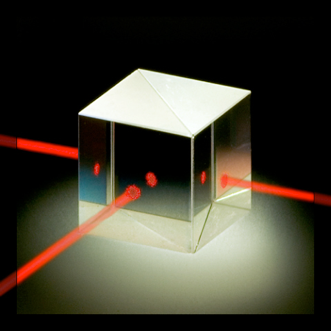
\includegraphics[scale=0.6]{./Bilder/Polarizer2.png}
\end{picture}
\caption{\label{fig_Pol}%
\textbf{a} Ein Polw\"urfel oder Polarisationsstrahlteiler
besteht aus zwei zusammengesetzten Prismen
mit einer besonders pr\"aparierten 
Grenzfl\"ache. \textbf{b} Ein einfallender
(unpolarisierter) Strahl wird in zwei (orthogonal)
polarisierte Strahlen aufgespalten. Der reflektierte
Strahl besitzt eine Polarisation parallel zur 
Grenzfl\"ache ($v$) -- in der Abbildung senkrecht
zur Bildebene --, der durchgelassene Strahl
eine horizontale Polarisation ($h$) in der Bildebene. 
\textbf{c} Umgekehrt kann
man auch zwei geeignet polarisierte Strahlen zu einem
gemeinsamen Strahl zusammenf\"uhren. Die Polarisation
des ausfallenden Strahls h\"angt von der relativen Phase
der beiden einfallenden Strahlen ab. Bei Phasengleichheit
ist der ausfallende Strahl linear polarisiert, an\-sons\-ten
elliptisch. Bei umgekehrter Wahl der Polarisationen f\"ur die
einfallenden Strahlen verl\"auft der ausfallende Strahl
in der Abbildung nach oben. (rechts) Abbildung eines Polarizationsstrahlteilers. (aus \cite{Filk} und \cite{?})}
\end{figure}

In der Abbildung wurde der Polarisationsw\"urfel so aufgestellt, dass der durchgelassene
Strahl eine horizontale Polarisation besitzt, der (um $90^\circ$) reflektierte Strahl eine
vertikale Polarisation. Der Polarisationsw\"urfel kann aber auch um die Achse des einfallenden
Strahls gedreht werden, sodass eine Aufspaltung in zwei orthogonale Polarisationsrichtungen
bez\"uglich jeder Orientierung des W\"urfels vorgenommen werden kann. 

Eine \glqq Messung\grqq\ mit einem solchen Polarisationsw\"urfel kann dadurch erfolgen,
dass hinter die beiden Austrittsrichtungen f\"ur den Lichtstrahl ein Detektor platziert wird,
der das austretende Licht nachweist. Ohne die Detektoren kann man mit dieser Anordnung
eine Polarisation pr\"aparieren: Man verwendet einfach den Strahl, der an der Seite zu
der gew\"unschten Polarisation austritt, f\"ur die weiteren Versuche. 

Nun ist bekannt, dass ein Lichtstrahl aus einer sehr gro\ss en Anzahl von Photonen bzw.\
Lichtquanten besteht. Ein Laserpointer strahlt pro Sekunde rund $10^{18}-10^{20}$ Photonen ab.
Wenn man die Intensit\"at eines Laserstrahls immer weiter verringert, gelangt man schlie\ss lich
zu einzelnen Photonen. In der Praxis l\"asst sich das schwer realisieren, da es aufgrund der
bosonischen Eigenschaften von Photonen zu sogenannten Bunching-Effekten kommt: Photonen
treten bevorzugt als Mehrfachpakete auf. Man erh\"alt also keine Einzelphotonen mit
nahezu konstanten Zeitabst\"anden zwischen ihnen. Auf dieses eher technische Detail soll hier aber
nicht weiter eingegangen werden. Es ist im Prinzip (mit hohem Kostenaufwand) m\"oglich,
gezielt Einzelphotonen herzustellen und f\"ur die optischen Experimente, die hier eine Rolle spielen,
zu verwenden. 

F\"ur Einzelphotonen gelten im Wesentlichen dieselben Regeln, wie f\"ur einen Lichtstrahl. Lediglich
die Gesetze bez\"uglich der Intensit\"at von Lichtstrahlen werden durch Gesetze f\"ur relative H\"aufigkeiten
- und im Fall von Einzelphotonen durch Wahrscheinlichkeiten - ersetzt. So besagt das Gesetz
von Malus, dass die Intensit\"at eines Lichtstrahls, der einen Polarisationsfilter unter einer Orientierung
zum Winkel $\alpha$ durchquert hat und durch einen zweiten Filter tritt, der unter dem Winkel $\beta$ orientiert
ist, um den Faktor $\cos^2 (\alpha - \beta)$ verringert wird. F\"ur einen Strahl mit $N$ Photonen hinter dem
ersten Filter lautet dieses Gesetz: F\"ur die Anzahl $N_1$ der Photonen, die auch den zweiten Filter passieren, gilt
ungef\"ahr: $N_1/N = \cos^2(\alpha - \beta)$. Und f\"ur ein Einzelphoton lautet das Gesetz: Die Wahrscheinlichkeit,
dass ein Photon, welches den ersten Filter passiert hat, auch den zweiten Filter passiert, ist $\cos^2(\alpha - \beta)$. 

Zur Beschreibung der Polarisation von Einzelphotonen verwenden wir wieder normierte Vektoren
in einem zweidimensionalen komplexen Vektorraum. Die horizontale und vertikale Polarisation beschreiben
wir meist durch die Einheitsvektoren aus Gl.\ \ref{eq_QM1_Basis}, wobei wir in der Notation die klassischen
Bitvariablen durch $h$ und $v$ ersetzen:
\begin{equation}
           |h\rangle = \left(\!\! \begin{array}{c}  1 \\ 0 \end{array}\!\! \right)  \hspace{1cm}
           |v\rangle = \left(\!\! \begin{array}{c}  0 \\ 1 \end{array} \!\!\right)  \, . 
\end{equation} 
Unter den Winkeln $+45^\circ$ und $-45^\circ$ polarisiertes Licht dr\"ucken wir entsprechend durch
$+$ und $-$ aus. In der obigen Basis gilt f\"ur die Vektoren zu dieser Polarisation:
\begin{equation}
           |+\rangle = \frac{1}{\sqrt{2}} \left(\!\! \begin{array}{c}  1 \\ 1 \end{array}\!\! \right)  \hspace{1cm}
           |-\rangle = \frac{1}{\sqrt{2}} \left(\!\! \begin{array}{c}  1  \\ - 1 \end{array}\!\! \right)  \, . 
\end{equation} 
Linear polarisiertes Licht kann man dadurch beschreiben, dass die allgemeinen Koeffizienten
in Gl.\ \ref{eq_QM1_Einheitsvektor} reell gew\"ahlt werden k\"onnen. Dies bringt zum Ausdruck, dass es
keine relative Phasenverschiebung zwischen den beiden Komponenten (horizontal und vertikal) gibt. 
Eine Polarisation unter einem allgemeinen Winkel $\theta$ relativ zur Horizontalen wird durch den
Vektor
\begin{equation}
           |\theta \rangle =  \left( \!\!\begin{array}{c}  \cos \theta \\ \sin \theta \end{array} \!\!\right)    
\end{equation} 
beschrieben.

Neben den linearen Polarisationen gibt es noch die zirkularen Polarisationen (und ganz allgemein die
elliptischen Polarisationen):
\begin{equation}
           |L\rangle = \frac{1}{\sqrt{2}} \left(\!\! \begin{array}{c}  1 \\ {\rm i} \end{array} \!\!\right)  \hspace{1cm}
           |R\rangle = \frac{1}{\sqrt{2}} \left(\!\! \begin{array}{c}  1  \\ - {\rm i} \end{array}\!\! \right)  \, . 
\end{equation} 
Hier spricht man von links zirkular polarisiertem Licht bzw.\ rechts zirkular polarisiertem Licht. 
Ganz allgemein kann eine Polarisation durch den Vektor
\begin{equation}
\label{eq_QM1_allgPol}
     |\theta, \delta \rangle =  \left( \!\!\begin{array}{c}  \cos \theta  \\ {\rm e}^{{\rm i}\delta} \, \sin \theta  \end{array} \!\!\right)    
\end{equation} 
gekennzeichnet werden. Da eine beliebige gemeinsame Phase f\"ur die beiden Komponenten
denselben Zustand beschreibt, kann die erste Komponente reell gew\"ahlt werden. Der Winkel
$\delta$ gibt die Elliptizit\"at der Polarisation an ($\delta=0$ entspricht linear polarisiertem Licht
und $\delta=\pm 90^\circ$ entspricht R- bzw.\ L-zirkular polarisiertem Licht) und der Winkel $\theta$ kennzeichnet die
Lage der gro\ss en Halbachse dieser Ellipse.  

\subsection{Die Menge der Observablen}

In diesem Abschnitt betrachten wir die Menge der hermiteschen Matrizen in dem zweidimensionalen
komplexen Vektorraum, die wir mit der Menge der Observablen identifizieren werden. Als Basis f\"ur die hermiteschen
Matrizen bieten sich die drei Pauli-Matrizen sowie die Einheitsmatrix an:
\begin{equation}
   {\bf 1} = \left( \begin{array}{cc}  1 & 0 \\ 0 & 1 \end{array} \right)  \hspace{0.7cm}
   \sigma_1  = \left( \begin{array}{cc}  0 & 1 \\ 1 & 0 \end{array} \right)  \hspace{0.7cm}
   \sigma_2  = \left( \begin{array}{cc}  0 & -{\rm i} \\ {\rm i} & 0 \end{array} \right)  \hspace{0.7cm}
   \sigma_3 = \left( \begin{array}{cc}  0 & 1 \\ 0 & -1 \end{array} \right)  \, .
\end{equation}
Diese vier Matrizen sind hermitesch (d.h.\ es gilt $A_{ij}=A^*_{ji}$). Eine beliebige reelle Linearkombination
ist ebenfalls hermitesch. Umgekehrt l\"asst sich jede hermitesche $2\times 2$-Matrix als reelle Linearkombination
in dieser Form schreiben:
\begin{equation}
      A = a_0 {\bf 1} + \sum_{i=1}^3 a_i \sigma_i = a_0 {\bf 1} + \pmb{a} \cdot \pmb{\sigma}_i
         =     \left( \begin{array}{cc}  a_0 + a_3 & a_1+{\rm i}a_2 \\ a_1 - {\rm i}_2 &  a_0 - a_3 \end{array} \right) \, .
\end{equation} 
\"Uber das charakteristische Polynom erh\"alt man die Eigenwerte $\lambda_i$:
\begin{equation}
\label{eq_QM1_Eigenwerte}
           \lambda_{1/2} = a_0 \pm \sqrt{a_1^2 + a_2^2 + a_3^2} = a_0 \pm | \pmb{a} |  \, .
\end{equation} 
$\sigma_1$ hat als Eigenvektoren $|+\rangle$ und $|-\rangle$, $\sigma_2$ hat als Eigenvektoren
$|R\rangle$ und $|L\rangle$ und $\sigma_3$ hat die Eigenvektoren $|h\rangle$ und $|v\rangle$. Da es
sich bei $A$ um eine selbst-adjungierte Matrix handelt, sind die Eigenvektoren von $A$ immer orthogonal
zueinander. Es handelt sich bei den Eigenvektoren einer Observablen also immer um zueinander orthogonale 
Polarisationsvektoren.

\subsection{Die Bloch-Kugel}

Die Bloch-Kugel veranschaulicht die m\"oglichen Polarisationszust\"ande. Aus Gl.\ \ref{eq_QM1_allgPol} wird schon
deutlich, dass man die Polarisationszust\"ande durch zwei Winkel $\theta$ und $\delta$ charakterisieren kann,
wobei $\theta \in [0,\pi]$ (nach einer Drehung um $180^\circ$ erh\"alt man dieselbe lineare Polarisation) 
und $\delta \in [-\pi,+\pi]$ (positive Vorzeichen entsprechen rechtszirkularen elliptischen Polarisationen und
negative Vorzeichen linkszirkularen). Diese Darstellung legt schon nahe, dass es sich bei der Menge der
Polarisationszust\"ande um eine Kugeloberfl\"ache handelt. 
Trotzdem ist die Identifikation der Winkelvariablen nicht so trivial.

Wie schon erw\"ahnt, lassen sich die (reinen) Zust\"ande auch durch eindimensionale Projektionsmatrizen darstellen, 
also hermitesche Matrizen mit der Eigenschaft $P^2=P$. Diese Eigenschaft l\"asst nur die Eigenwerte 1 und 0 zu.
Ist ein Eigenwert 1 und der andere 0, projizieren diese
Matrizen auf eindimensionale Unterr\"aume. Aus Gl.\ \ref{eq_QM1_Eigenwerte} erkennt man, dass diese beiden
Eigenwerte nur in folgendem Fall auftreten:
\begin{equation}
      a_0 = \frac{1}{2}   \hspace{1cm} {\rm und} \hspace{1cm}  |\pmb{a}| = \frac{1}{2} \, .
\end{equation}
In zwei Dimensionen k\"onnen wir also jede Projektionsmatrix auf einen eindimensionalen Unterraum 
in der Form
\begin{equation}
         P =  \frac{1}{2} \Big( {\bf 1} + \pmb{n} \cdot \pmb{\sigma} \Big) 
\end{equation}
schreiben, wobei $\pmb{n}$ ein beliebiger 3-dimensionaler Einheitsvektor ist. Damit wird deutlich, dass sich jeder Zustand
durch einen 3-dimensionalen Einheitsvektor darstellen l\"asst. Diese Darstellung bezeichnet man als 
Bloch-Kugel (siehe Abb.\ \ref{fig_Bloch}).\footnote{Henri Poincar\'{e} hat schon 1892 diese Darstellung f\"ur die Polarisationszust\"ande
von Licht verwendet, daher wird sie in der Optik auch als Poincar\'{e}-Kugel bezeichnet.}

\begin{SCfigure}[50][htb]
\begin{picture}(200,180)(0,0)
\qbezier(20,90)(20,122)(43.4,146.6)
\qbezier(43.4,146.6)(68,170)(100,170)
\qbezier(20,90)(20,58)(43.4,33.4)
\qbezier(43.4,33.4)(68,10)(100,10)
\qbezier(180,90)(180,122)(156.6,146.6)
\qbezier(156.6,146.6)(132,170)(100,170)
\qbezier(180,90)(180,58)(156.6,33.4)
\qbezier(156.6,33.4)(132,10)(100,10)
%
\qbezier(20,90)(20,110)(100,110)
\qbezier(20,90)(20,70)(100,70)
\qbezier(100,110)(180,110)(180,90)
\qbezier(100,70)(180,70)(180,90)
%
\put(20,90){\line(1,0){160}}
\put(80,70.5){\line(1,1){39}}
\put(100,10){\line(0,1){160}}
%
\put(20,90){\makebox(0,0){$\bullet$}}
\put(100,10){\makebox(0,0){$\bullet$}}
\put(100,170){\makebox(0,0){$\bullet$}}
\put(180,90){\makebox(0,0){$\bullet$}}
\put(80,70.5){\makebox(0,0){$\bullet$}}
\put(120,109.5){\makebox(0,0){$\bullet$}}
\put(100,90){\makebox(0,0){$\bullet$}}
%
\put(10,90){\makebox(0,0){$|h \rangle$}}
\put(190,90){\makebox(0,0){$|v \rangle$}}
\put(100,2){\makebox(0,0){$|L \rangle$}}
\put(100,178){\makebox(0,0){$|R \rangle$}}
\put(80,62.5){\makebox(0,0){$| - \rangle$}}
\put(120,117.5){\makebox(0,0){$| + \rangle$}}
\put(114,83){\makebox(0,0){$\rho=\frac{1}{2}{\bf 1}$}}
\end{picture}
\caption{\label{fig_Bloch}%
Die Bloch-Kugel f\"ur Polarisationszust\"ande von Licht. Die Kugeloberfl\"ache
repr\"asentiert die reinen Zust\"ande, das Kugelinnere die gemischten
Zust\"ande. Gegen\"uberliegende Punkte (Antipoden) entsprechen orthogonalen Polarisationszust\"anden.}
\end{SCfigure}

F\"ur den Fall $|\pmb{n}|<1$ erh\"alt man sogenannte Dichtematrizen. Sie beschreiben gemischte
Zust\"ande aus verschiedenen Polarisationen. Der Spezialfall $|\pmb{n}|=0$ f\"uhrt auf die Einheitsmatrix
(multipliziert mit $1/2$). In diesem Fall kann keine Aussage \"uber die Polarisation getroffen werden bzw.\
alle Polarisationsrichtungen sind gleich wahrscheinlich. Dies ist der maximal gemischte Zustand. Das 
Innere der Bloch-Kugel kennzeichnet somit gemischte Zust\"ande, die Oberfl\"ache die reinen Zust\"ande. 

Man beachte, dass die Bloch-Kugel in einem 3-dimensionalen reellen Vektorraum liegt. Orthogonale
Polarisationen ($h$ und $v$ oder $+$ und $-$ oder auch $L$ und $R$) liegen auf der Bloch-Kugel antipodisch
gegen\"uber. Es handelt sich bei diesem Vektorraum daher nicht um den Hilbert-Raum der Zust\"ande, in dem
orthogonale Polarisationen auch durch orthogonale Vektoren dargestellt werden.

\section{Verschr\"ankung}

Ebenso wie in der klassischen Informationstheorie interessiert man sich in der Quanteninformation
nicht nur f\"ur einzelne QuBits, sondern f\"ur Ketten bzw.\ Folgen von QuBits. Im Folgenden betrachten wir
nur QuBit-Paare, also Systeme zur Darstellung von zwei QuBits. Es zeigt sich, dass man auch in der
Quantentheorie (\"ahnlich wie in der klassischen Informationstheorie) die meisten Operationen auf
QuBit-Folgen als Hintereinanderausf\"uhrung von Operationen auf QuBit-Paaren darstellen kann. 

Ein System aus zwei QuBits (z.B.\ die Polarisationszust\"ande von zwei Photonen) wird im Tensorprodukt
der beiden einzelnen zweidimensionalen Vektorr\"aume beschrieben. Man erh\"alt auf diese Weise einen
vierdimensionalen komplexen Vektorraum. In einem solchen Tensorprodukt
beschreibt man die Vektoren gerne mit Doppelindizes. So ist bespielsweise das Tensorprodukt aus
einem Vektor $\pmb{x}$ und einem Vektor $\pmb{y}$ gegeben durch:
\begin{equation}
\label{eq_QM1_Tensor}
       \pmb{x} \otimes \pmb{y} = \left( \begin{array}{c} x_1 \\ x_2 \end{array} \right) \otimes
          \left( \begin{array}{c} y_1 \\ y_2 \end{array} \right) =
           \left( \begin{array}{c} x_1 y_1  \\ x_1 y_2 \\ x_2 y_1 \\ x_2 y_2  \end{array} \right)
%           \simeq  \left( \begin{array}{cc} x_1 y_1 &  x_1 y_2 \\ x_2 y_1 & x_2 y_2  \end{array} \right)  
            \, .
\end{equation}
Das Tensorprodukt der beiden Vektorr\"aume besteht aus allen Linearkombinationen solcher
Vektoren, wobei folgendes Distributivgesetz gilt:\footnote{Man beachte den Unterschied zur
direkten Summe von Vektorr\"aumen bzw.\ Vektoren:
\[      (\pmb{x}_1 + \pmb{x}_2) \oplus (\pmb{y}_1 + \pmb{y}_2) = \pmb{x}_1  \oplus \pmb{y}_1 +
     \pmb{x}_2  \oplus \pmb{y}_2  \, . \]  
und $\pmb{0} \oplus \pmb{y}$ sowie $\pmb{x}\oplus \pmb{0}$ sind von null verschiedene Vektoren. Statt
$\pmb{x} \oplus \pmb{y}$ schreibt man hier oft einfacher $(\pmb{x},\pmb{y})$.}
\begin{equation}
     (\pmb{x}_1 + \pmb{x}_2) \otimes (\pmb{y}_1 + \pmb{y}_2) = \pmb{x}_1  \otimes \pmb{y}_1 +
     \pmb{x}_1  \otimes \pmb{y}_2 +\pmb{x}_2  \otimes \pmb{y}_1 +\pmb{x}_2  \otimes \pmb{y}_2 
\end{equation}
sowie
\begin{equation}
     \pmb{0} \otimes \pmb{y} = \pmb{x} \otimes \pmb{0} = \pmb{0} \, .
\end{equation}

Man erkennt sofort, dass in Gl.\ \ref{eq_QM1_Tensor} das Produkt der beiden \"au\ss eren Komponenten 
(die erste und vierte Komponente) gleich dem 
Produkt der beiden inneren Komponenten ist. Dies kennzeichnet den Vektor (in zwei Dimensionen) eindeutig
als separabel, wobei ein Vektor in dem vierdimensionalen Vektorraum als separabel bezeichnet wird, wenn
es zwei Vektoren $\pmb{x}$ und $\pmb{y}$ in den einzelnen Vektorr\"aumen gibt, sodass sich der
vierdimensionale Vektor als Tensorprodukt der beiden zweidimensionalen Vektoren schreiben l\"asst. 
Falls das nicht m\"oglich ist - allgemein sich also ein Vektor in einem Tensorproduktraum nicht als Tensorprodukt
von zwei Vektoren in den einzelnen Vektorr\"aumen schreiben l\"asst - bezeichnet man den Vektor
als verschr\"ankt. In zwei Dimensionen haben wir somit ein einfaches Kriterium f\"ur die Verschr\"anktheit
von zwei Vektoren: Wenn das Produkt der ersten und vierten Komponente eines Vektors nicht gleich dem
Produkt der zweiten und dritten Komponente ist, ist der Vektor verschr\"ankt. 

Bei Wellenfunktionen zu zwei Teilsystemen (oder allgemeiner zu zwei unabh\"angigen Klassen von
Freiheitsgraden), die durch Funktionen von zwei Variablen beschrieben werden, bedeutet Separierbarkeit,
dass $\Psi(x,y)= \varphi(x) \psi(y)$. Die Wellenfunktion l\"asst sich also als einfaches Produkt von zwei
Funktionen darstellen. F\"ur verschr\"ankte Wellenfunktionen gilt das nicht. 

Man beachte, dass der Begriff der Verschr\"anktheit nur sinnvoll ist, wenn f\"ur einen Vektorraum eine
Zerlegung als ein Tensorprodukt definiert ist. Ohne die Angabe einer solchen Produktdarstellung ist
der Begriff der Verschr\"ankung nicht definiert. Die Angabe einer solchen Produktdarstellung gibt an,
in welcher Form das Gesamtsystem als aus zwei Teilsystemen bestehend gedacht werden kann. Bei
zwei Teilchen ist eine solche Zerlegung physikalisch naheliegend (jedes Teilchen definiert sein Teilsystem). 
Es kann jedoch auch eine Verschr\"ankung beispielsweise zwischen den Polarisationsfreiheitsgraden
eines Photons und seinen r\"aumlichen Eigenschaften bestehen. So hat ein einzelnes Photon, das
durch einen Doppelspalt tritt, wobei hinter dem rechten Spalt ein $+$-Polarisationsfilter und hinter dem
linken Spalt ein $-$-Polarisationsfilter steht, eine Verschr\"ankung zwischen seiner Polarisation und dem
Spalt, durch den es getreten ist. Der Zustand
\begin{equation}
        | \gamma \rangle = \frac{1}{\sqrt{2}} \Big( |+\rangle \otimes |r \rangle + |- \rangle \otimes |l\rangle \Big)
\end{equation}
beschreibt ein solches Photon. Die $+$-Polarisation ist korreliert mit dem rechten Spalt und die $-$-Polarisation
mit dem linken. Dieser Zustand ist im Sinne der obigen Definition verschr\"ankt. Die Darstellung des Zustands
einzelner Photonen durch solche Verschr\"ankungen
zwischen ihrem Polarisationsfreiheitsgrad und ihrer r\"aumlichen Eigenschaft ist
ganz sinnvoll, beispielsweise bei der Beschreibung von Experimenten zum Quantenradierer. Meistens hat man es aber mit
Verschr\"ankungen zwischen den Polarisationszust\"anden (bzw.\ allgemeiner den zwei Zust\"anden) 
eines Systems aus zwei Teilchen zu tun. 

Die physikalische Bedeutung der Verschr\"ankung liegt unter anderem an folgender Eigenschaft 
verschr\"ankter Zust\"ande. Ist ein Zustand separierbar, so separiert auch das Absolutquadrat 
der Komponenten des Vektors, durch den der Zustand beschrieben wird (vgl.\ Gl.\ \ref{eq_QM1_Tensor}).
Diese Absolutquadrate entsprechen aber nach der Born'schen Regel 
bei Einzelsystemen den Wahrscheinlichkeiten, dass 
zwei Ereignisse gleichzeitig auftreten (bei Funktionenr\"aumen handelt es sich um Wahrscheinlichkeitsdichten,
die zur Berechnung einer Wahrscheinlichkeit \"uber ein Volumen zu integrieren sind). Beispielsweise ist
in Gl.\ \ref{eq_QM1_Tensor} $w_{ij}=|x_i|^2|y_j|^2$ die Wahrscheinlichkeit f\"ur das gleichzeitige Auftreten der
beiden Ereignisse $i$ und $j$. Faktorisierende
Wahrscheinlichkeiten f\"ur zwei Ereignisse bedeutet aber, dass diese Ereignisse unkorreliert sind. 
Eine Information \"uber das Vorliegen eines der beiden Ereignisse \"andert nichts an der Wahrscheinlichkeit
f\"ur das Auftreten des zweiten Ereignisses. 

Bei verschr\"ankten Zust\"anden ist dies anders: Erh\"alt man eine Information \"uber das Vorliegen eines
Ereignisses beispielsweise an einem Teilsystem, kann man neue Vorhersagen \"uber das Eintreffen eines 
anderen Ereignisses an dem anderen Teilsystem treffen. Im Extremfall liegt das Ereignis an dem anderen
Teilsystem sogar eindeutig fest. Dies ist dann besonders erstaunlich, wenn die beiden Teilsysteme
sehr weit voneinander entfernt sind. Weshalb sollte eine Messung an einem Teilsystem auf der Erde
eine instantane Ver\"anderung des anderen Teilsystems im Andromeda-Nebel zur Folge haben? Diese
Eigenschaft verschr\"ankter Zust\"ande h\"angt eng mit der Problematik der Lokalit\"at der Quantentheorie
zusammen. 

\section{Bell-Zust\"ande}

In dem Tensorproduktraum von zwei Zwei-Zustandssystemen gibt es eine ausgezeichnete Basis, die man erh\"alt,
wenn man die Tensorprodukte der Basisvektoren in den einzelnen Hilbert-R\"aumen bildet:
\begin{equation}
           |h\rangle \otimes |h\rangle = \left( \begin{array}{c}  1 \\ 0 \\ 0 \\ 0 \end{array} \right) \hspace{0.4cm}
           |h\rangle \otimes |v\rangle = \left( \begin{array}{c}  0 \\ 1 \\ 0 \\ 0 \end{array} \right) \hspace{0.4cm}
           |v\rangle \otimes |h\rangle = \left( \begin{array}{c}  0 \\ 0 \\ 1 \\ 0 \end{array} \right) \hspace{0.4cm}
           |v\rangle \otimes |v\rangle = \left( \begin{array}{c}  0 \\ 0 \\ 0 \\ 1 \end{array} \right) \, .
\end{equation}
Diese Basisvektoren sind alle separabel. Zur Beschreibung von verschr\"ankten Zust\"anden bietet es sich
oft an, eine Basis zu w\"ahlen, bei der alle Basisvektoren maximal verschr\"ankt sind.\footnote{Es gibt eine
technische Definition von maximal verschr\"ankt: Wenn die Spur \"uber die Projektionsmatrix des Zustands 
\"uber einen der Teilr\"aume die Identit\"atsmatrix in dem verbliebenen Teilraum ergibt. Physikalischer
ausgedr\"uckt: Ein Zustand hei\ss t maximal verschr\"ankt, wenn der Erwartungswert f\"ur beliebieg 
Messungen an einem Teilsystem durch eine Dichtematrix proportional zur Identit\"atsmatrix - also maximale
Unkenntnis - beschrieben werden muss. Dies wird im Folgenden
aber nicht ben\"otigt.} Die Orthonormalbasis aus den folgenden vier Zust\"anden hat diese Eigenschaft.
Diese Zust\"ande bezeichnet man als Bell-Zust\"ande:
\begin{eqnarray}
      |\Phi^+ \rangle &=&  \frac{1}{\sqrt{2}} \Big( |h\rangle \otimes |h\rangle + |v\rangle \otimes |v\rangle \Big)
            = \frac{1}{\sqrt{2}} \left( \begin{array}{c}  1 \\ 0 \\ 0 \\ 1 \end{array} \right)   \\[0.2cm]  
      |\Phi^- \rangle &=&  \frac{1}{\sqrt{2}} \Big( |h\rangle \otimes |h\rangle - |v\rangle \otimes |v\rangle \Big)
            = \frac{1}{\sqrt{2}} \left( \begin{array}{c}  1 \\ 0 \\ 0 \\ -1 \end{array} \right)   \\[0.2cm]
      |\Psi^+ \rangle &=&  \frac{1}{\sqrt{2}} \Big( |h\rangle \otimes |v\rangle + |v\rangle \otimes |h\rangle \Big)
            = \frac{1}{\sqrt{2}} \left( \begin{array}{c}  0 \\ 1 \\ 1 \\ 0 \end{array} \right)   \\[0.2cm]  
      |\Psi^- \rangle &=&  \frac{1}{\sqrt{2}} \Big( |h\rangle \otimes |v\rangle - |v\rangle \otimes |h\rangle \Big)
            = \frac{1}{\sqrt{2}} \left( \begin{array}{c}  0 \\ 1 \\ - 1 \\ 0 \end{array} \right)    \, .
\end{eqnarray}
Den letzten Zustand, $|\Psi^- \rangle$, bezeichnet man auch oft als EPR-Zustand (nach Einstein-Podolsky-Rosen). 
Er hat einige besondere Eigenschaften, insbesondere liegt die Antikorrelation bez\"uglich jeder Basis vor, d.h.\
es gilt:
\begin{equation}
  |{\rm EPR} \rangle = \frac{1}{\sqrt{2}} \Big( |h\rangle \otimes |v\rangle - |v\rangle \otimes |h\rangle \Big) 
  = \frac{1}{\sqrt{2}} \Big( |+\rangle \otimes |-\rangle - |-\rangle \otimes |+\rangle \Big) =
    \frac{1}{\sqrt{2}} \Big( |R\rangle \otimes |L\rangle - |L\rangle \otimes |R\rangle \Big) \, .
\end{equation}
Es handelt sich bei diesem Bell-Zustand um den Eigenzustand zum Gesamtdrehimpuls 0 (Photonen haben einen
Spin 1, und zwei Photonen k\"onnen sich zum Gesamtspin 0 oder Gesamtspin 2 verbinden). Dieser Zustand
ist invariant unter Drehungen und daher in allen Basissystemen formgleich. F\"ur den Zustand $|\Phi^+\rangle$
gilt diese Eigenschaft, sofern man sich auf lineare Polarisationen beschr\"ankt.
 


\begin{thebibliography}{99}
\bibitem{Aspect} Aspect, A., Grangier, Ph., Roger, G.; 
       {Experimental Realization of Einstein-Podolsky-Rosen-Bohm 
        Gedankenexperiment: A New Violation of Bell's Inequalities}; 
        Phys.\ Rev.\ Lett.\ 49 (1982) 91--94. \\
        Aspect, A., Dalibard, J., Roger, G.; {Experimental Test 
        of Bell's Inequalities Using Time-Varying Analyzers}; 
        Phys.\ Rev.\ Lett.\ 49 (1982) 1804--1807.
\bibitem{Bell} Bell, J.; {\em Against \glq Measurement\grq};
        in {\em 62 Years of Uncertainty}, Erice, 5--14 August 1989;
        auch in {\em Physics World} 8 (1990) 33--40. Abgedruckt in
        \cite{Bell2}. 
\bibitem{Bell2} Bell, J.S.;  {\em Speakable and Unspeakable in 
        Quantum Physics}, 2.\ edition, Cambridge University Press (2004).         
        \bibitem{Filk} Filk, T; \textit{Quantenmechanik (nicht nur) f\"ur Lehramtsstudierende}; Springer-Verlag, 2019.
\bibitem{Schroedinger} Schr\"odinger, E.; {\em Die gegenw\"artige
        Situation in der Quantenmechanik}; Die Naturwissenschaften 23
        (1935) 807--812, 823--828,  844-849.      
\end{thebibliography}

\end{document}

